\section{Auswertung}

\subsection{Bestimmung der Schallgeschwindigkeit mit dem Puls-Echo-Verfahren}

\begin{table}[H] 
\centering 
\caption{Daten zur Bestimmung der Schallgeschwindigkeit in Acryl mit der Impuls-Echo-Methode. Laufstrecke $s$, Zeitlicher Abstand der Pulse zum Ursprung $t_1$, $t_2$ und berechnete halbe Zeitdifferenz $\frac{\Delta t }{2}$.} 
\label{tab: c_echo} 
\begin{tabular}{S S S S } 
\toprule  
{$s / \si{\milli\meter}$} & {$t_1 / \si{\micro\second}$} &  {$t_2 / \si{\micro\second}$}& {$\frac{\Delta t }{2} / \si{\micro\second}$}  \\ 
\midrule  
 31.10  & 0.4  & 23.9  & 11.8\\ 
40.00  & 0.3  & 29.8  & 14.8\\ 
61.68  & 0.4  & 46.3  & 22.9\\ 
72.00  & 1.1  & 53.4  & 26.1\\ 
80.60  & 1.1  & 59.8  & 29.3\\ 
111.78  & 1.3  & 82.6  & 40.6\\ 
120.80  & 1.3  & 88.9  & 43.8\\ 
\bottomrule 
\end{tabular} 
\end{table}

\begin{figure}[H]
  \centering
  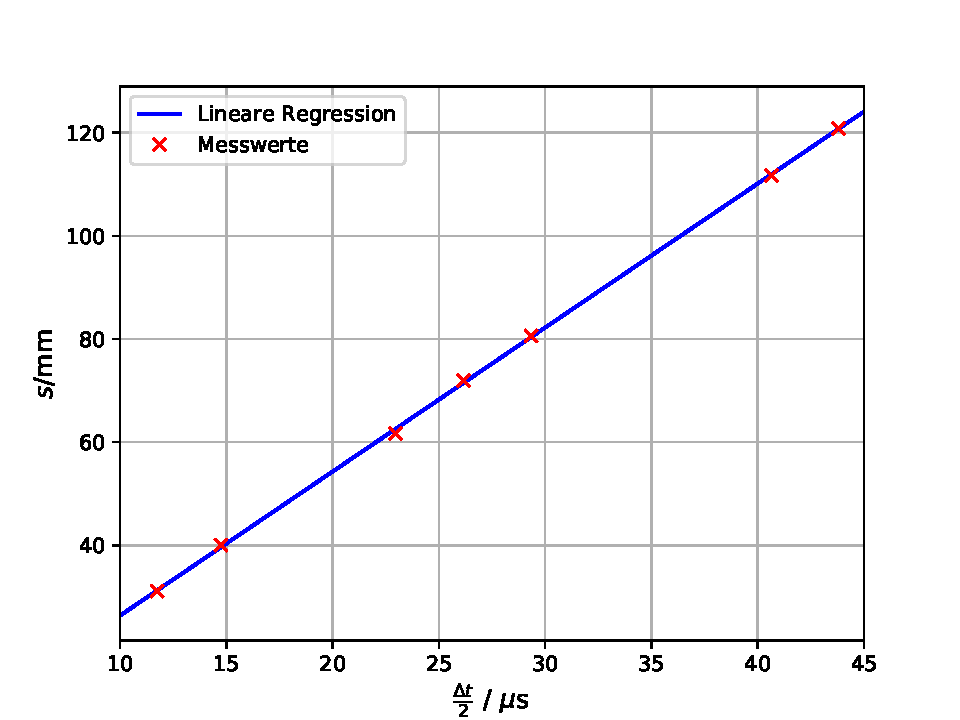
\includegraphics[width = 0.7\textwidth]{../Messdaten/plots/schallgeschwindigkeit.pdf}
  \caption{Graphische Darstellung der Messwertpaare zur Bestimmung der Schallgeschwindigkeit
  mit der Impuls-Echo-Methode (Strecke $s$ und Laufzeit $\frac{\Delta t}{2}$) sowie der linearen Regression.}
  \label{fig: c_echo}
\end{figure}


\subsection{Bestimmung der Schallgeschwindigkeit mit dem Durchschallungsverfahren}

\begin{table} 
\centering 
\caption{Daten zur Bestimmung der Schallgeschwindigkeit in Acryl mit der Durchschallungsmethode. Laufstrecke $s$ und Laufzeit $t$.} 
\label{tab: c_durchsschallung} 
\begin{tabular}{S S } 
\toprule  
{$s / \si{\milli\meter}$} & {$t / \si{\micro\second}$}  \\ 
\midrule  
 31.10  & 12.9\\ 
40.00  & 15.8\\ 
61.68  & 23.9\\ 
80.60  & 30.5\\ 
102.36  & 39.2\\ 
120.80  & 45.3\\ 
\bottomrule 
\end{tabular} 
\end{table}

\begin{figure}[H]
  \centering
  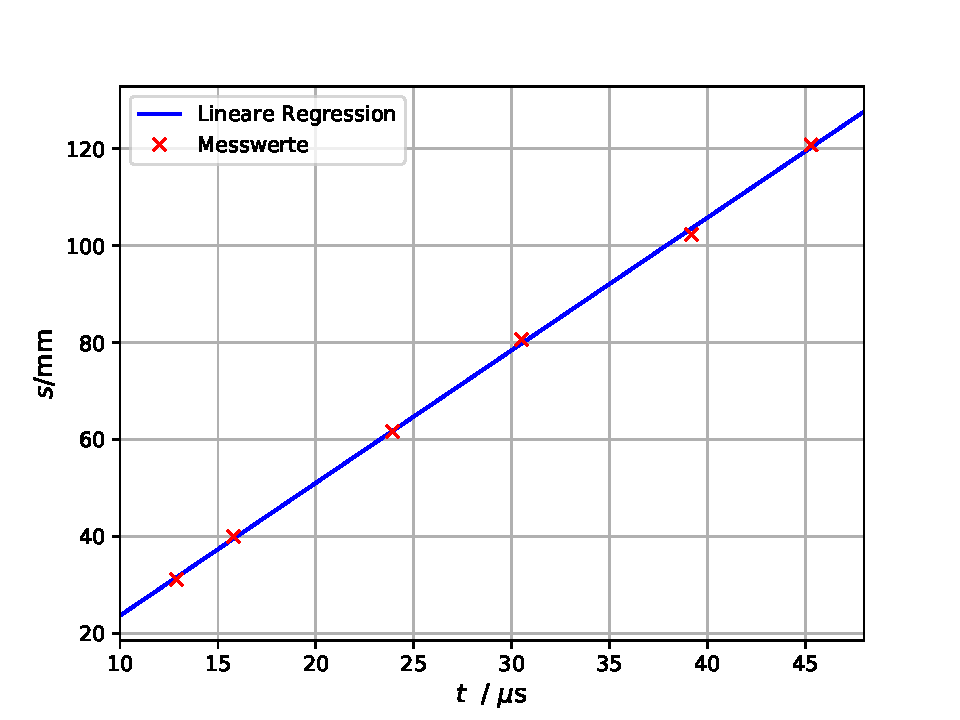
\includegraphics[width = 0.7\textwidth]{../Messdaten/plots/schallgeschwindigkeit_durchschallung.pdf}
  \caption{Graphische Darstellung der Messwertpaare zur Bestimmung der Schallgeschwindigkeit
  mit der Durchschallungsmethode (Strecke $s$ und Laufzeit $t$) sowie der linearen Regression.}
  \label{fig: c_durchsschallung}
\end{figure}


\subsection{Bestimmung der Dämpfungskonstante}


\subsection{Spektrale Analyse}
Die graphische Darstellung des aufgenommenen Cepstrums ist in Abbildung \ref{fig: cepstrum} einzusehen.
Die zeitlichen Koordinaten der erkennbaren Spannungspulse sind in Tabelle \ref{} eingetragen und ebenfalls in
Abbildung \ref{} dargestellt. Aus den halben Differenzen und der gemittelten Schallgeschwindigkeit \ref{} berechnen sich die
Dicken der Acrylplatten zu
\begin{align}
  \begin{aligned}
    p_1 &= \SI{+12.02(7)}{\milli\meter}\\
    p_2 &= \SI{+12.30(8)}{\milli\meter}.
  \end{aligned}
\end{align}
Das aufgenommene Spektrum ist in Graphik \ref{fig: spektrum} einzusehen. Von einer genauen Untersuchung des Ergebnisses wird abgesehen, da
die erkennbaren Peaks zu schlecht voneinander zu differenzieren sind. Eine qualitative Betrachtung erfolgt in der Diskussion.
\begin{figure}[H]
  \centering
  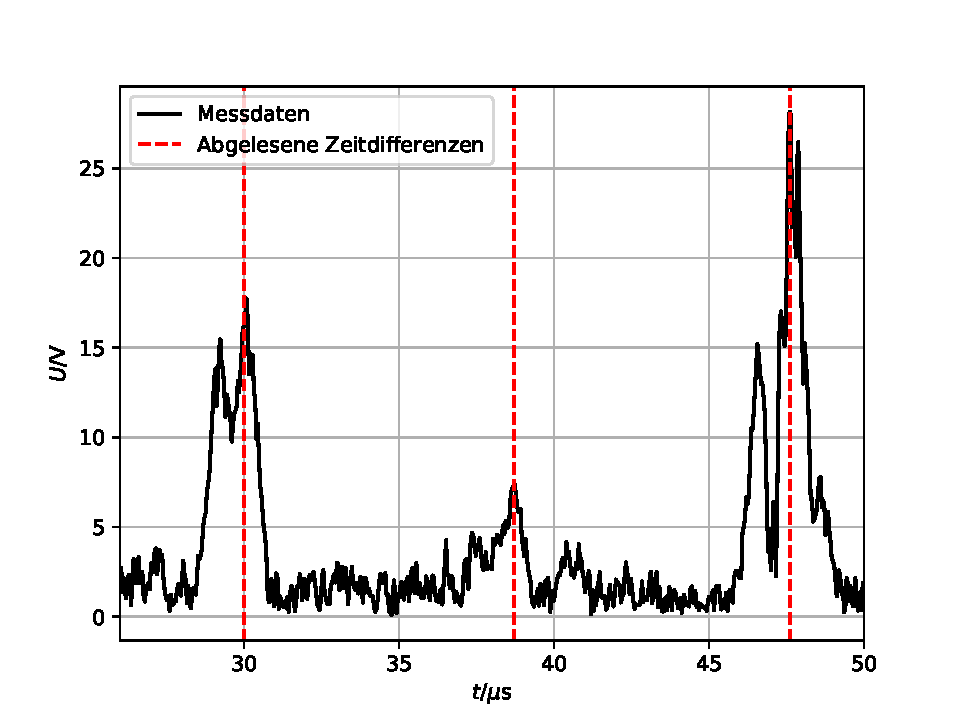
\includegraphics[width = 0.7\textwidth]{../Messdaten/plots/cepstrum.pdf}
  \caption{Graphische Darstellung des Cepstrums. Zeitliche Differenz $t$ und Amplitude $U$.}
  \label{fig: cepstrum}
\end{figure}

\begin{figure}[H]
  \centering
  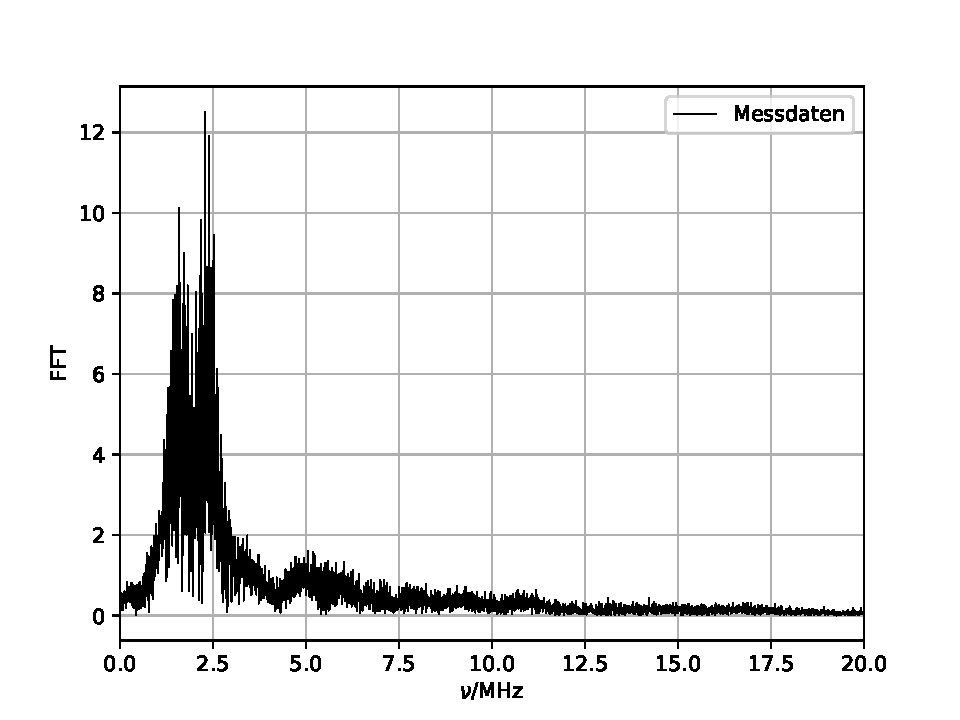
\includegraphics[width = 0.7\textwidth]{../Messdaten/plots/spectrum.pdf}
  \caption{Spektrum. Frequenz $\nu$ und FFT.}
  \label{fig: spektrum}
\end{figure}

\subsection{Längenmessung am Augenmodell}
Die aufgenommenen Daten zur Längenmessung am Augenmodell sind in Abbildung \ref{fig: auge} dargestellt. Die mit Hilfe
der Messsoftware bestimmten zeitlichen Koordinaten der erkennbaren Peaks sind in Tabelle \ref{} aufgeführt, sowie in Abbildung
\ref{fig: auge} eingezeichnet. Mit der gemittelten Schallgeschwindigkeit \ref{} und den halben zeitlichen Differenzen zwischen den
Peaks ergeben sich folgende räumliche Abstände
\begin{align}
  \begin{aligned}
  a_1 &= \SI{+13.41(8)}{\milli\meter}\\
  a_2 &= \SI{+7.19(4)}{\milli\meter}\\
  a_3 &= \SI{+9.40(6)}{\milli\meter}\\
  a_4 &= \SI{+68.8(4)}{\milli\meter}.
\end{aligned}
\end{align}


\begin{figure}[H]
  \centering
  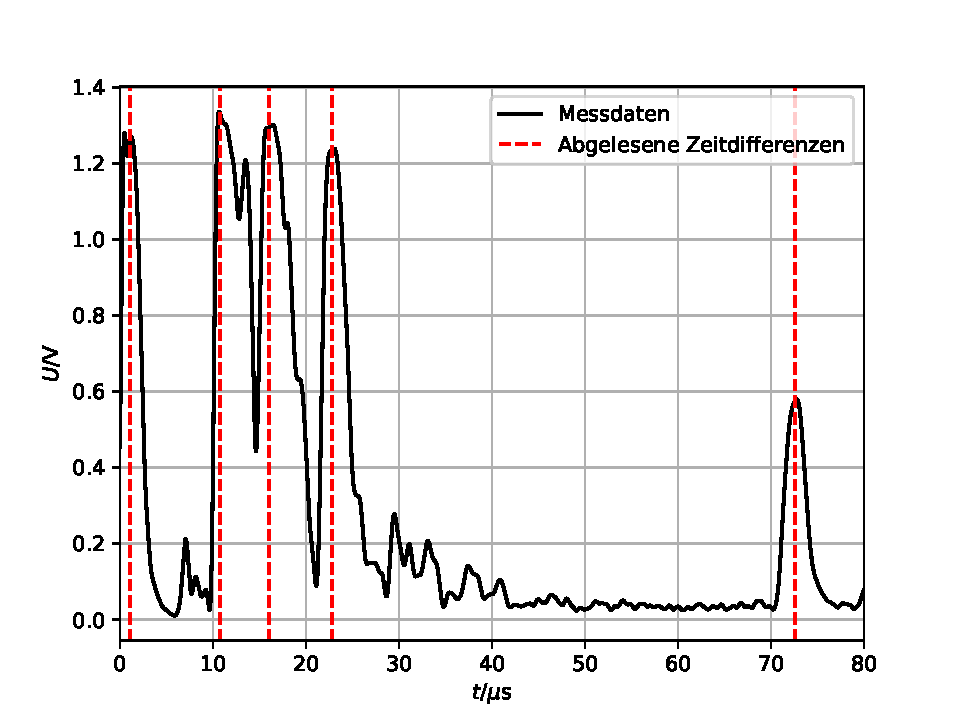
\includegraphics[width = 0.7\textwidth]{../Messdaten/plots/auge.pdf}
  \caption{Graphische Darstellung der aufgenommenen Messwerte zur Untersuchung des Augenmodells. Zeitlicher Abstand $t$ und Amplitude $U$.}
  \label{fig: auge}
\end{figure}
